\subsection{Blinn-Phong Model}

\begin{frame}{Blinn-Phong: A More Efficient Alternative}
  \begin{columns}
    \begin{column}{0.6\textwidth}
      \begin{raybox}{Motivation for Blinn-Phong}
        \footnotesize
        \textbf{Problem with Phong:} Computing the reflection vector $\mathbf{R}$ is expensive
        \begin{align*}
          \mathbf{R} = 2(\mathbf{N} \cdot \mathbf{L})\mathbf{N} - \mathbf{L}
        \end{align*}

        \vspace{0.3cm}
        \pause
        \textbf{Jim Blinn's solution (1977):} Use a halfway vector instead

        \vspace{0.3cm}
        \pause
        \textbf{Key insight:}
        \begin{itemize}
          \item When $\mathbf{V} = \mathbf{R}$, the halfway vector $\mathbf{H}$ equals the normal $\mathbf{N}$
          \item We can measure the angle between $\mathbf{H}$ and $\mathbf{N}$ instead
          \item Much cheaper to compute!
        \end{itemize}
      \end{raybox}
    \end{column}
    \begin{column}{0.4\textwidth}
      \begin{tikzpicture}[scale=0.8]
        % Surface
        \draw[ObjectColor, very thick] (-2,0) -- (2,0);
        \fill[ObjectColor] (0,0) circle (3pt);
        \draw[->, PrimaryColor, thick] (0,0) -- (0,1.5) node[above,black] {\footnotesize $\mathbf{N}$};
        \draw[->, lightray, thick] (0,0) -- (135:1.5) node[left,black] {\footnotesize $\mathbf{L}$};

        \draw[->, AccentColor, thick] (0,0) -- (15:1.5) node[right] {\footnotesize $\mathbf{V}$};

        \draw[->, PrimaryColor, thick] (0,0) -- (45:1.5) node[right] {\footnotesize $\mathbf{R}$};

        \only<2->{
          \draw[->, red, very thick] (0,0) -- (75:1.5) node[right] {\footnotesize $\mathbf{H}$};

          \node[below] at (0,-0.5) {\footnotesize Halfway vector bisects};
          \node[below] at (0,-0.8) {\footnotesize $\mathbf{L}$ and $\mathbf{V}$};

          \draw[-] (0, 1) arc [start angle=90, end angle=75, radius=1cm];
        }
      \end{tikzpicture}
    \end{column}
  \end{columns}
\end{frame}

\begin{frame}{Blinn-Phong Mathematics and Comparison}
  \begin{columns}
    \begin{column}{0.5\textwidth}
      \begin{mathbox}{Blinn-Phong Formula}
        \footnotesize
        \textbf{Halfway vector calculation:}
        \begin{align}
          \mathbf{H} = \frac{\mathbf{L} + \mathbf{V}}{|\mathbf{L} + \mathbf{V}|}
        \end{align}

        \textbf{Specular term:}
        \begin{align}
          I_{\text{spec}} = \mathbf{k}_s \odot \mathbf{I}_l \max(0, \mathbf{N} \cdot \mathbf{H})^{n'}
        \end{align}

        where $n'$ is typically 2-4 times larger than Phong's $n$

        \vspace{0.3cm}
        \pause
        \textbf{Performance comparison:}
        \begin{itemize}
          \item \textbf{Phong:} 5 operations (2 dot products, 1 scalar multiply, 2 vector ops)
          \item \textbf{Blinn-Phong:} 4 operations (1 vector add, 1 normalize, 1 dot product)
        \end{itemize}
      \end{mathbox}
    \end{column}
    \begin{column}{0.5\textwidth}
      \begin{figure}
        \centering
        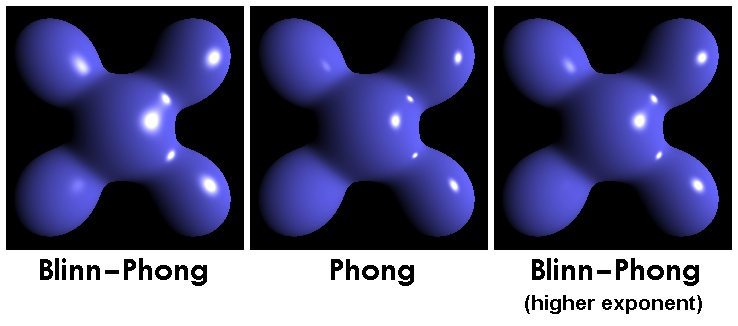
\includegraphics[width=0.9\linewidth]{images/blinn-phong.png}
        \caption*{\scriptsize Blinn-Phong vs Phong}
      \end{figure}
    \end{column}
  \end{columns}
\end{frame}